\chapter{Einleitung}
\thispagestyle{fancy}
\label{chap:Einleitung}
\pagenumbering{arabic}

Die \ac{ATS} ist dem Bereich des \ac{NLP} zuzuordnen und gewinnt zunehmend an wissenschaftlicher Relevanz. Obgleich entsprechende Modelle mittlerweile nicht mehr völlig neuartig sind, weisen die Entwicklungen der vergangenen Jahre qualitativ noch viele Potenziale auf. Modelle sind prinzipiell als das Ergebnis des Trainingsprozesses neuronaler Netze zu verstehen. Einsatzmöglichkeiten entsprechender \ac{ATS}Modelle sind beispielsweise die Zusammenfassung von Nachrichten, die Zusammenfassung von Gesprächsprotokollen oder auch die Generierung von Überschriften, um nur wenige zu nennen \cite{GON20, GAM16}. Ziel ist in jedem Fall die Verdichtung von Informationen und die Reduktion der Lesezeit.\\

Mit besonderem Fokus auf das Gesundheitswesen lassen sich weiterhin zwei konkrete Einsatzgebiete konstruieren, in denen ein \ac{ATS}-Modell in einem ganzheitlichen System als autarkes Modul implementiert werden könnte. Einerseits ist die Zusammenfassung von Patientengesprächen denkbar, wenn eine entsprechende Spracherkennung mit integrierter Sprechererkennung vorgeschaltet ist. Die verdichteten Informationen ließen sich anschließend zum Beispiel in Patientenakten exportieren oder anderweitig klassifizieren. Andererseits können Pflegeroboter, welche mitunter demente Patienten betreuen, durch ein \ac{ATS}-Modell mit notwendigem Kontextwissen für die anstehenden Gespräche ausgestattet werden.\\

Die Anforderungen an ein \ac{ATS}-Modell lassen sich aus dem individuell avisierten Einsatzgebiet ableiten und können anhand verschiedener Faktoren klassifiziert werden, wie \autoref{pic:Systemtypen} veranschaulicht.\\
- TODO: Inhalt der Grafik niederschreiben, Quelle weiterhin referenzieren, dann Grafik entfernen

\begin{figure}
  \centering
  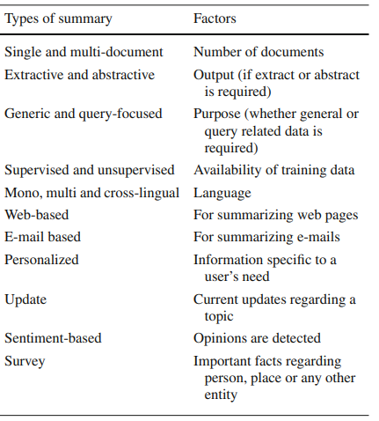
\includegraphics[scale=0.8]{./source/images/systemtypen.jpg}
  \caption{Typen von Zusammenfassungen \cite{GAM16}}
  \label{pic:Systemtypen}
\end{figure}

Aus technischer Sicht kommen grundsätzlich sogenannte Sequence-to-Sequence-Modelle zum Einsatz. Dabei wird stets eine Eingabesequenz $x = [x_{1}, ..., x_{n}]$ in eine Ausgabesequenz $y = [y_{1}, ..., y_{m}]$ überführt, wobei $n$ die Eingabelänge und $m$ die Ausgabelänge ist. Mithin wird bei der \ac{ATS} $m$ \textless \, $n$ intendiert. Entsprechende Architekturen modellieren also konsequenterweise die Wahrscheinlichkeit $P(y \mid x)$. Die maßgebliche Herausforderung ist hierbei zum einen, dass \ac{ATS}-Modelle tatsächlich die wichtigsten Informationen einer Eingabesequenz identifizieren. Zum anderen gilt es, diese Informationen in eine entsprechende Ausgabesequenz zu integrieren. Eben diese Ausgabesequenz ist zudem orthographisch und grammatikalisch korrekt zu generieren.\\

% \section{MediaInterface GmbH \& SpeaKING\textsuperscript{\textregistered}}


\section{Zielsetzung}
Das Ziel dieser Arbeit ist dementsprechend die abstraktive Zusammenfassung einzelner Dokumente, wobei multilingual vortrainierte Modelle mittels \ac{TL} auf die deutsche Sprache adaptiert werden. Die Arbeit ist somit außerdem eine potenzielle Grundlage für die beiden konstruierten Einsatzgebiete aus dem Gesundheitswesen. Die Adaption auf die Domäne oder auch die Dialogorientierung sind nicht Teil dieser Arbeit. Die Forschungsfragen lauten wie folgt:

\begin{itemize}
	\item Wie lassen sich Texte automatisiert zusammenfassen?
	\item Wie können bereits existierende Modelle auf eine andere Sprache adaptiert werden?
	\item Wie qualitativ und skalierbar ist die Lösung?
\end{itemize}


\section{Aufbau der Arbeit}
Nach der Einleitung werden zunächst die Grundlagen des \ac{DL} und des \ac{NLP} offengelegt. Im Kapitel des \ac{DL} werden neuronale Netze als solches definiert und ausgewählte Architekturen, welche auf die Zielerreichung einwirken, vorgestellt. Die Eigenschaften und die Relevanz von Hyperparametern und von \ac{TL} schließen sich an. Im Kapitel des \ac{NLP} werden neben der prinzipiellen Arbeit mit natürlicher Sprache und der entsprechenden Vorverarbeitung insbesondere sogenannte Word Embeddings und Deep Language Representations thematisiert. Bevor die bis dahin behandelten Komponenten in ein tatsächliches Modell integriert werden können, ist die Beschreibung der Datengrundlage erforderlich. Zum daran anschließenden abstraktiven Ansatz gehört die Erläuterung der Architektur, die Beschreibung des Trainingsprozesses und die Evaluation der Ergebnisse. Bei der sprachtechnischen Adaption des Modells auf die deutsche Sprache werden zuerst entsprechende Anpassungen an der ursprünglichen Architektur konzipiert, bevor erneut der Trainingsprozess beschrieben wird und die dazugehörigen Ergebnisse evaluiert werden.


\section{Forschungsstand \& Referenzen}
Notizen:
\begin{itemize}
	\item NLP-SOTA beschreiben, ggf. Übergriff zu anderen interdisziplinären Anwendungsgebieten andeuten, hier genutzte Datensätze, welche als Benchmark dienen und die zur Verbesserung des Scores genutzt werden könnten, sind: \url{https://paperswithcode.com/task/abstractive-text-summarization}, \url{https://paperswithcode.com/task/text-summarization}, also CNN/ Daily-Mail, Wikihow und Gigaword
	\item Vergleichbare Arbeiten beschreiben (vgl. Paper: „German Abstractive Text Summarization using Deep Learning“ und „Automatic Text Summarization“)
	\item Kürzlich entwickelte Ansätze (vgl. Paper: „Recent Automatic Text Summarization Techniques“)
	\item SOTA-Modelle recherchieren (vgl. Paper: „Automatic Text Summarization“ und weitere Architekturen aus dem Internet, ggf. auch ohne zugehöriges Paper)
	\item Nützliche GitHub-Repo's verlinken/ referenzieren und deren hauptsächliche Herangehensweise dokumentieren, hierfür siehe GitHub-Stars und Notizen nachfolgender Kapitel
	\item Medizinische Zusammenfassung: \url{https://github.com/armancohan/long-summarization}
	\item Architekturen: \url{https://towardsdatascience.com/deep-learning-models-for-automatic-summarization-4c2b89f2a9ea}, \url{https://medium.com/analytics-vidhya/deep-reinforcement-learning-deeprl-for-abstractive-text-summarization-made-easy-tutorial-9-c6914999c76c}, \url{https://github.com/yaserkl/RLSeq2Seq#dataset}, \url{https://medium.com/analytics-vidhya/deep-reinforcement-learning-deeprl-for-abstractive-text-summarization-made-easy-tutorial-9-c6914999c76c}, \url{https://github.com/rohithreddy024/Text-Summarizer-Pytorch}, \url{https://github.com/oceanypt/A-DEEP-REINFORCED-MODEL-FOR-ABSTRACTIVE-SUMMARIZATION}, \url{https://github.com/theamrzaki/text_summurization_abstractive_methods}
	\item Möglicherweise als Paper aufnehmen, oder sogar für spätere Kapitel nutzen: \url{https://arxiv.org/abs/1805.11080, https://arxiv.org/pdf/1705.04304v3.pdf}, gleiche Prüfung stets auch bei andere URL's in den Notizen dieser Arbeit durchführen
	\item Vergleich verschiedener Modelle anhand des ROUGE-Scores: \url{http://nlpprogress.com/english/summarization.html}, in den Ergebnissen erwähnen, Korpus-Zusammensetzung beachten
	\item SOTA: CNN \url{https://paperswithcode.com/sota/abstractive-text-summarization-on-cnn-daily}, Wikihow \url{https://paperswithcode.com/sota/abstractive-text-summarization-on-wikihow}
\end{itemize}
